\begin{figure}[!htb]
    \centering

    \tikzstyle{arrow} = [rounded corners, line width = 1mm, bend left = 15, ->]
    
    \resizebox{0.85\width}{!}{
    \begin{tikzpicture}[node distance=1cm]
        
        \node (information) {
\includegraphics[width=.15\textwidth]{Fundamentação/Fatores Humanos/thinking.png}} 
        node(t_information)[below of = information,yshift=-0.75cm] {Information}
        node(t_information2)[below of = t_information,yshift=0.25cm] {processing};
        
        \node (controlling) [right of=information, xshift=5cm, yshift=-3cm] {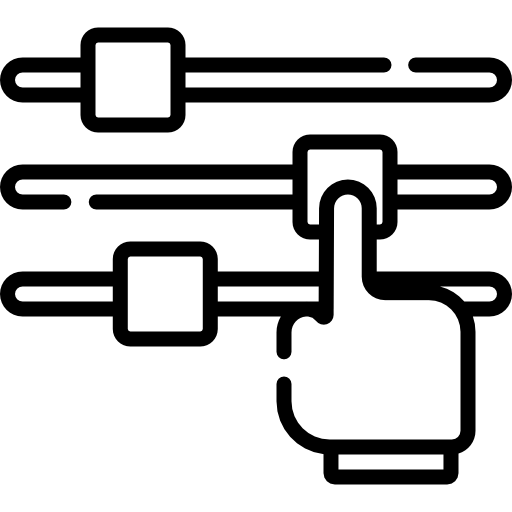
\includegraphics[width=.15\textwidth]{Fundamentação/Fatores Humanos/slider.png}}
        node(t_controlling)[below of = controlling,yshift = -0.75cm] {Controlling};
        
        \node (controls) [below of=controlling, yshift=-5cm,] {
\includegraphics[width=.15\textwidth,angle=90,origin=c]{Fundamentação/Fatores Humanos/control.png}} 
        node(t_controls) [below of = controls, yshift = -0.75cm]{Controls};
        
        \node (machine) [left of=controls, xshift=-5cm, yshift=-2cm] {
\includegraphics[width=.15\textwidth]{Fundamentação/Fatores Humanos/machine.png}} 
        node(t_machine) [below of = machine, yshift = -0.75cm]{Operation};
        
        \node (display) [left of=machine, xshift=-5cm, yshift=2cm] {
\includegraphics[width=.15\textwidth]{Fundamentação/Fatores Humanos/monitor.png}} 
        node(t_display) [below of = display, yshift = -0.75cm]{Display};
        
        \node (senses) [left of=information, xshift=-5cm, yshift=-2cm,] {\begin{tikzpicture}[node distance=1cm]
    \centering
    
    \node (eye) {
\includegraphics[width=.075\textwidth]{Fundamentação/Fatores Humanos/eye.png}};
    
    \node (ear) [right of=eye, yshift=-0.65cm] {
\includegraphics[width=.075\textwidth]{Fundamentação/Fatores Humanos/ear.png}};
    
    \node (nose) [left of=ear, yshift=-0.65cm] {
\includegraphics[width=.075\textwidth]{Fundamentação/Fatores Humanos/nose.png}};
    
    \node (hand) [right of=nose, yshift=-0.85cm] {
\includegraphics[width=.075\textwidth]{Fundamentação/Fatores Humanos/hand.png}};

\end{tikzpicture}} 
        node(t_senses) [below of = senses, yshift = -1.25cm]{Senses};
        
        \node (human) [below of=information, yshift=-4.75cm] {\Large{Human}};
        \node (human) [above of=machine, yshift=3.25cm] {\Large{Machine}};
        \node (human) [above of=information, yshift=1cm] {\Large{Work Environment}};
        
        \node (left_point) [left of=display, xshift=-2, yshift=2.75cm] {};
        \node (right_point) [right of=left_point, xshift=14cm] {};
        
        \node (input) [left of=machine, xshift=-5cm, yshift=-2cm] {\Large{Input}};
        \node (output) [right of=machine, xshift=5cm, yshift=-2cm] {\Large{Output}};
        
    
        \draw [arrow] (information.east) to (controlling.north west);
        \draw [arrow] (t_controlling.south) to (controls.north);
        \draw [arrow] (controls.west) to (machine.east);
        \draw [arrow] (machine.west) to (display.east);
        \draw [arrow] (display.north) to (t_senses.south);
        \draw [arrow] (senses.east) to (information.west);
        \draw [arrow] (input.east) -- (machine);
        \draw [arrow] (machine) -- (output.west);
        \draw [dashed,gray] (left_point) to (right_point);
        
        \draw (-8,-14) rectangle(8cm,1.5cm);
        
    \end{tikzpicture}
    }
    \caption{Human-Machine system representation. Adapted from \cite{sanders1998human}.}
    \label{fig:human_machine_representaion}
\end{figure}